%
%
\begin{centered}
Le plan est muni d'un repère $\OIJ$.
\end{centered}
%
%
%
%----------------------------------------------
%
\section{Les fonctions affines}
%
%----------------------------------------------
%
\subsection{Définitions et caractérisation}
%
%
%
\begin{dfn}
Une fonction $f$ définie sur $\R$ est dite \emph{affine} lorsqu'il existe deux réels $m$ et $p$  tels que :
    \begin{centered}
    pour tout $x \in \R$, $f(x)=mx+p$.
    \end{centered}
 
Dans ce cas, $m$ est le \emph{coefficient directeur} de $f$ et $p$ est \emph{l'ordonnée à l'origine} de $f$.
\end{dfn}
%
%
%
\begin{dfn} Soit $f$ une fonction affine telle que $f(x)=mx+p$.
\begin{itemize}
\item Si $m=0$ alors $f\colon x\mapsto p$ est une fonction \emph{constante}.
\item Si $p=0$ alors $f\colon x\mapsto mx$ est une fonction \emph{linéaire}.
\end{itemize}
\end{dfn}
%
%\begin{prp}{}{}
%Une fonction $f$ est une fonction linéaire \ssi* $ f(x_1+x_2)=f(x_1)+f(x_2)$ pour tous réels $x_1$ et $x_2$.
%\end{prp}
%
% 
%\begin{prp}{}{} Une fonction linéaire est représentée par une droite \emph{passant par~l'origine}.
%\end{prp}
%
%
% \begin{rmq}{}{}
%\begin{itemize}
% \item Une fonction linéaire est aussi une fonction affine (pour laquelle $b=0$).
%\item \textbf{Attention :} la majorité des fonctions ne sont pas linéaires, à commencer par les fonctions affines $x\mapsto ax+b$ telles que $b\neq0$ !%, la fonction carrée, \dots
% \end{itemize}
%\end{rmq}
%
%
%
\begin{prp} Soit $f$ une fonction définie sur $\R$. 

$f$ est une fonction affine \ssi pour tous réels $a$ et $b$ distincts, $\dfrac{f(b)-f(a)}{b-a}$ est constant.
\end{prp}
%
%
%
Le nombre $\dfrac{f(b)-f(a)}{b-a}$ s'appelle le taux d'accroissement de $f$ entre $a$ et $b$.
%
%
%
\begin{prp}
Soit $f$ la fonction affine définie par $f(x)=mx+p$ et $a$ et $b$ deux réels distincts.
\begin{itemize}
\item Le coefficient directeur de $f$ est le taux d'accroissement de $f$ : $m=\dfrac{f(b)-f(a)}{b-a}$.
\item L'ordonnée à l'origine est $p=f(a)-m\times a$. En particulier, $p=f(0)$.
\end{itemize}
\end{prp}
%
%----------------------------------------------
%
\subsection{Représentation graphique}
%
%----------------------------------------------
%
\begin{prp}
\begin{itemize}
\item La représentation graphique d'une fonction affine est une droite sécante avec $\Oy$ (droite \og{}oblique\fg{}).
\item Réciproquement, une droite sécante avec $\Oy$ est la représentation graphique d'une fonction affine.
\end{itemize}
\end{prp}

Soit $f$ la fonction affine définie par $f(x)=mx+p$ et $\droite*{D}$ sa représentation graphique.
\begingroup
\makeatletter
% Strongly encourage LaTeX not to break before this list.
% http://tex.stackexchange.com/a/46795/1680
\@endparpenalty=10000
\makeatother
    \begin{itemize}
    \item On dit que la droite $\droite*{D}$ a pour équation $y=mx+p$.
\hfill\def\CoefDir{0.6}
\def\OrdOrig{0.7}
\def\SbDebPente{0.6}
\def\SbLgPente{1}
\begin{tikzpicture}
\path[use as bounding box] (-1.5,2.75) -- (2.3,2.75);
\tkzInit[xmin=-1.5,xstep=1,xmax=2.2,ymin=-0.5,ystep=1,ymax=2]
\tkzDrawX[line width=0.75pt,noticks,color=black,label={x}]
\tkzDrawY[up space=0.2,line width=0.75pt,noticks,color=black,label={y}]
\tkzFct[line width=0.75pt,domain =-2:3]{0+(\CoefDir)*(\x)+(\OrdOrig)}   %
\FPadd\resultt\SbDebPente\SbLgPente
\tkzDefPointByFct(\SbDebPente) \tkzGetPoint{C}%
\tkzDefShiftPoint[C](\SbLgPente,0){D}
\tkzDefPointByFct(\resultt) \tkzGetPoint{E}%
\tkzSetUpPoint[shape=cross out,size=4]
\tkzDefPoint(0,\OrdOrig){B}
\tkzDrawPoints(B,C,E)
%\tkzLabelPoint[below=1ex](M){$-\dfrac{b}{a}$}
\tkzLabelPoint[left=1ex](B){$p$}
\tkzDrawSegments[dashed](C,D D,E)
\tkzLabelSegment[below,pos=.5](C,D){$1$}
\tkzLabelSegment[right,pos=.5](D,E){$m$}
\end{tikzpicture}

    Cela signifie que pour tout point $N$ du plan, $N\in\droite*{D}$ \ssi $y_N=m\times x_N+p$.
    \item Soient $A$ et $B$ deux points distincts de $\droite*{D}$.

    Le \emph{coefficient directeur} de $\droite*{D}$ est $m=\dfrac{y_B-y_A}{x_B-x_A}$. 
%    
    Il est indépendant des points $A$ et $B$ choisis.
    \item \emph{L'ordonnée à l'origine} $p$ de $\droite*{D}$ est l'ordonnée du point de $\droite*{D}$ d'abscisse 0. 
    
    C'est l'ordonnée du point d'intersection de $(D)$ et $\Oy$.
    \item Pour tracer $(D)$ on peut :
        \begin{itemize}
        \item  utiliser deux points $A\cord{x_A;y_A}$ et $B\cord{x_B;y_B}$ tels que $y_A=ax_A+b$ et $y_B=ax_B+b$.% (il faut choisir $x_A$ et $x_B$ et calculer $y_A$ et $y_B$).
        \item utiliser l'ordonnée à l'origine et le coefficient directeur. 
        \end{itemize}
    \end{itemize}
\endgroup

\begin{att}
Une droite parallèle à $\Oy$ n'est la représentation d'aucune fonction.
\end{att}
%
%----------------------------------------------
%
\pagebreak
\section{\'Etude d'une fonction affine}
%
%----------------------------------------------
%
%
%\subsection{Parité}
%%
%%
%\begin{prp}
%Soit $f$ une fonction affine.
%\begin{itemize-}(2)
%\item $f$ est impaire \ssi $f$ est une fonction linéaire.
%\item  $f$ est paire \ssi $f$ est constante.
%\end{itemize-}
%\end{prp}
%
%
\subsection{Variations}
%
%
\begin{prp}{}{} Soit une fonction affine $f\colon x\mapsto mx+p$.
\begin{itemize}
\item Si $m<0$ alors $f$ est (strictement) \hfill\dots\hfill: \hfill
\begin{tikzpicture}[y=0.9cm,align at top]
\tikzset{arrow style/.style={black,%
					line width=0.75pt,->,%
					>= latex',%
					shorten >= 6pt,%
					shorten <= 6pt}}
\tkzTabInit[lgt=1.5,espcl=3]%,deltacl=0.4
{$x$/0.5,$f(x)$/1.25}{$-\infty$,$+\infty$}%
%\tkzTabVar{+/ ,-/ }%
\end{tikzpicture}
\item Si $m>0$ alors $f$ est (strictement)  \hfill\dots\hfill: \hfill
\begin{tikzpicture}[y=0.9cm,align at top]
\tikzset{arrow style/.style={black,%
					line width=0.75pt,->,%
					>= latex',%
					shorten >= 6pt,%
					shorten <= 6pt}}
\tkzTabInit[lgt=1.5,espcl=3]%,deltacl=0.4
{$x$/0.5,$f(x)$/1.25}{$-\infty$,$+\infty$}%
%\tkzTabVar{-/ ,+/ }%
\end{tikzpicture}
\item Si $m=0$ alors $f$ est  \hfill\dots\hfill: \hfill
\begin{tikzpicture}[y=0.9cm,align at top]
\tikzset{arrow style/.style={black,%
					line width=0.75pt,->,%
					>= latex',%
					shorten >= 6pt,%
					shorten <= 6pt}}
\tkzTabInit[lgt=1.5,espcl=3]%,deltacl=0.4
{$x$/0.5,$f(x)$/1}{$-\infty$,$+\infty$}%
%\draw[arrow style] ($(N11)!0.5!(N12)$) --  ($(N21)!0.5!(N22)$);
\end{tikzpicture}
\end{itemize}
\end{prp}
%
%
%
\begin{intgr}{}{}~\newline% 
\begin{minipage}[c]{\linewidth}\vspace*{2ex}
\noindent\begin{minipage}[c]{0.3\linewidth}
\centering
Lorsque $m<0$ :\vspace*{1ex}

\noindent\def\CoefDir{-0.65}
\def\OrdOrig{1.3}
\def\SbDebPente{0.5}
\def\SbLgPente{1}
\begin{tikzpicture}[scale=1]
\tkzInit[xmin=-1,xstep=1,xmax=3.5,ymin=-1.2,ystep=1,ymax=2]
\tkzDrawX[line width=0.75pt,noticks,color=black,label={x}]
\tkzDrawY[up space=0.2,line width=0.75pt,noticks,color=black,label={y}]
\tkzFct[samples=100,line width=0.75pt,domain =-1:3.5]{0+(\CoefDir)*(\x)+(\OrdOrig)}   %
\tkzDefPointByFct(3.2)
\tkzText[anchor=east,left=3pt](tkzPointResult){$(d)$}
\FPdiv\Result\OrdOrig\CoefDir
\FPadd\resultt\SbDebPente\SbLgPente
\tkzDefPointByFct(\SbDebPente) \tkzGetPoint{C}%
\tkzDefShiftPoint[C](\SbLgPente,0){D}
\tkzDefPointByFct(\resultt) \tkzGetPoint{E}%
\tkzSetUpPoint[shape=cross out,size=4]
\tkzDefPointByFct[draw](-\Result) \tkzGetPoint{M}%
\tkzDefPoint(0,\OrdOrig){B}
\tkzDrawPoints(M,B)
%\tkzLabelPoint[below=1ex](M){$-\dfrac{b}{a}$}
\tkzLabelPoint[left,anchor=north east](B){$p$}
\tkzDrawSegments[dashed](C,D D,E)
\tkzLabelSegment[above,pos=.5](C,D){$1$}
\tkzLabelSegment[right,pos=.5](D,E){$m$}
\end{tikzpicture}
\end{minipage}
\hfill
\vrule
\hfill
\begin{minipage}[c]{0.3\linewidth}
\centering
Lorsque $m>0$ :\vspace*{1ex}

\def\CoefDir{0.65}
\def\OrdOrig{0.8}
\def\SbDebPente{0.4}
\def\SbLgPente{1}
\begin{tikzpicture}[scale=1]
\tkzInit[xmin=-2.6,xstep=1,xmax=1.9,ymin=-1.2,ystep=1,ymax=2]
\tkzDrawX[line width=0.75pt,noticks,color=black,label={x}]
\tkzDrawY[up space=0.2,line width=0.75pt,noticks,color=black,label={y}]
\tkzFct[samples=100,line width=0.75pt,domain =-2.6:1.9]{0+(\CoefDir)*(\x)+(\OrdOrig)}   %
\tkzDefPointByFct(-2.5)
\tkzText[below,right=4pt](tkzPointResult){$(d)$}
\FPdiv\Result\OrdOrig\CoefDir
\FPadd\resultt\SbDebPente\SbLgPente
\tkzDefPointByFct(\SbDebPente) \tkzGetPoint{C}%
\tkzDefShiftPoint[C](\SbLgPente,0){D}
\tkzDefPointByFct(\resultt) \tkzGetPoint{E}%
\tkzSetUpPoint[shape=cross out,size=4]
\tkzDefPointByFct[draw](-\Result) \tkzGetPoint{M}%
\tkzDefPoint(0,\OrdOrig){B}
\tkzDrawPoints(M,B)
%\tkzLabelPoint[below=1ex](M){$-\dfrac{b}{a}$}
\tkzLabelPoint[left=1ex](B){$p$}
\tkzDrawSegments[dashed](C,D D,E)
\tkzLabelSegment[below,pos=.5](C,D){$1$}
\tkzLabelSegment[right,pos=.5](D,E){$m$}
\end{tikzpicture}
\end{minipage}
\hfill
\vrule
\hfill
\begin{minipage}[c]{0.3\linewidth}
\centering
Lorsque $m=0$ :\vspace*{1ex}

\noindent\begin{tikzpicture}[scale=1]
\tkzInit[xmin=-2.5,xstep=1,xmax=2,ymin=-1.2,ystep=1,ymax=2]
\tkzDrawX[line width=0.75pt,noticks,color=black,label={x}]
\tkzDrawY[up space=0.2,line width=0.75pt,noticks,color=black,label={y}]
\tkzFct[samples=100,line width=0.75pt,domain =-2.5:2]{1}   %
\tkzDefPointByFct(1.25)
\tkzText[above](tkzPointResult){$(d)$}
\end{tikzpicture}
\end{minipage}
\end{minipage}
\end{intgr}

On en déduit la propriété suivante :
\vspace*{5pt}\begin{prp}{}{}
\begin{enumerate}
\item En ajoutant (ou retranchant) un même nombre aux deux membres d'une inégalité, on obtient une inégalité de même sens. %Autrement dit, $b$ étant un réel : 
%$x>y \ssi$ \hspace{1em}\pointille{1em}%$x+b>y+b$.
\item En multipliant (ou divisant) les deux membres d'une inégalité par un même nombre strictement positif, on obtient une inégalité de même sens. %Autrement dit, $a$ étant un réel \emph{strictement positif} : 
%$x>y \ssi$ \hspace{1em}\pointille{1em}%$ax>ay$.
\item En multipliant (ou divisant) les deux membres d'une inégalité par un même nombre strictement négatif, on obtient une inégalité de sens contraire.% Autrement dit, $a$ étant un réel \emph{strictement négatif} : \newline
%$x>y \ssi$ \hspace{1em}\pointille{1em}%$ax<ay$.
\end{enumerate}
\end{prp}
%
%
%
\subsection{Signes}
%
%
\begin{prp}{}{} Soit une fonction affine $f\colon x\mapsto mx+p$.
\begin{itemize}
\item Si $m<0$ alors : \hspace*{0.5cm}
\begin{minipage}[c]{0.7\linewidth}
{\centering
\begin{tikzpicture}
\tkzTabInit[lgt=3,espcl=3]{$x$ /0.75%
				, signe de $f(x)$ /0.75}%
{$-\infty$,\dots,$+\infty$}%
\tkzTabLine{ , \dots , z ,\dots , }
\end{tikzpicture}

} 
\end{minipage}
  \item Si $m>0$ alors : \hspace*{0.5cm}
\begin{minipage}[c]{0.7\linewidth}
{\centering
\begin{tikzpicture}
\tkzTabInit[lgt=3,espcl=3]{$x$ /0.75%
				, signe de $f(x)$ /0.75}%
{$-\infty$,\dots,$+\infty$}%
\tkzTabLine{ , \dots , z , \dots , }%\noexpand\pointille{$-\frac{p}{m}$}
\end{tikzpicture}

}
\end{minipage}
\end{itemize}
\end{prp}